% \documentclass[a4paper,10pt]{article}
% \usepackage[utf8]{inputenc}
% \usepackage{geometry}
% \usepackage[table]{xcolor}
% \usepackage{colortbl}
% \usepackage{color,soul}
% \geometry{margin=0.8in}
% \usepackage{xcolor}
% \usepackage{tikz}
% \usepackage{minted}
% \definecolor{bgcolor}{rgb}{0.8, 0.9, 0.5} % 
% \definecolor{bgcolor1}{rgb}{0.95, 0.95, 0.95} % Light Gray
% \definecolor{bgcolor2}{rgb}{0.85, 0.92, 1.0}  % Soft Blue
% \definecolor{bgcolor3}{rgb}{0.9, 0.85, 1.0}   % Light Purple
% \definecolor{bgcolor4}{rgb}{0.95, 0.88, 0.76} % Warm Beige
% \definecolor{bgcolor5}{rgb}{0.8, 0.95, 0.8}   % Gentle Green
% \definecolor{bgcolor6}{rgb}{1.0, 0.87, 0.87}  % Pastel Red
% \definecolor{bgcolor7}{rgb}{0.86, 0.93, 0.83} % Mint Green
% \definecolor{bgcolor8}{rgb}{0.98, 0.85, 0.94} % Soft Pink
% \definecolor{bgcolor9}{rgb}{0.87, 0.94, 0.98} % Sky Blue
% \definecolor{bgcolor10}{rgb}{0.96, 0.96, 0.82} % Pale Yellow
% 
% \begin{document}
\section*{Graphs Problem Solutions}
\noindent\textbf{Problem: Breadth First Traversal (BFS)}
\begin{minted}[
bgcolor=bgcolor4,
frame=lines,
framesep=5mm,
rulecolor=\color{black},
linenos,
numbersep=5pt,
fontsize=\normalsize
]{python}
from collections import deque
def bfs(graph: dict, start: int) -> List[int]:
    """
    Performs BFS traversal starting from given node.
    Time Complexity: O(V+E)    Space Complexity: O(V)
    """
    visited = set([start])
    queue = deque([start])
    result = []
    
    while queue:
        node = queue.popleft()
        result.append(node)
        for neighbor in graph[node]:
            if neighbor not in visited:
                visited.add(neighbor)
                queue.append(neighbor)
    return result
\end{minted}

\noindent\textbf{Problem: Depth First Traversal (DFS)}
\begin{minted}[
bgcolor=bgcolor2,
frame=lines,
framesep=5mm,
rulecolor=\color{black},
linenos,
numbersep=5pt,
fontsize=\normalsize
]{python}
def dfs(graph: dict, start: int) -> List[int]:
    """
    Performs DFS traversal (recursive) from given node.
    Time Complexity: O(V+E)    Space Complexity: O(V)
    """
    visited = set()
    result = []
    
    def dfs_util(node):
        visited.add(node)
        result.append(node)
        for neighbor in graph[node]:
            if neighbor not in visited:
                dfs_util(neighbor)
    
    dfs_util(start)
    return result
\end{minted}

\noindent\textbf{Problem: Shortest Path in Unweighted Graph}
\begin{minted}[
bgcolor=bgcolor5,
frame=lines,
framesep=5mm,
rulecolor=\color{black},
linenos,
numbersep=5pt,
fontsize=\normalsize
]{python}
from collections import deque
def shortest_path_unweighted(graph: dict, start: int, end: int) -> List[int]:
    """
    Finds shortest path in unweighted graph using BFS.
    Time Complexity: O(V+E)    Space Complexity: O(V)
    """
    queue = deque([start])
    visited = {start: None}  # Store parent pointers
    
    while queue:
        node = queue.popleft()
        if node == end:
            break
        for neighbor in graph[node]:
            if neighbor not in visited:
                visited[neighbor] = node
                queue.append(neighbor)
    
    # Reconstruct path
    path = []
    if end not in visited:
        return path
    while end is not None:
        path.append(end)
        end = visited[end]
    return path[::-1]
\end{minted}

\noindent\textbf{Problem: Shortest Path in DAG (Topo Sort)}
\begin{minted}[
bgcolor=bgcolor7,
frame=lines,
framesep=5mm,
rulecolor=\color{black},
linenos,
numbersep=5pt,
fontsize=\normalsize
]{python}
def shortest_path_dag(graph: dict, n: int, start: int) -> List[int]:
    """
    Finds shortest paths from start node in DAG using topological sort.
    Time Complexity: O(V+E)    Space Complexity: O(V)
    """
    # Topological sorting using Kahn's algorithm
    indegree = [0] * n
    for node in graph:
        for neighbor in graph[node]:
            indegree[neighbor] += 1
    
    queue = deque()
    for i in range(n):
        if indegree[i] == 0:
            queue.append(i)
    
    topo = []
    while queue:
        node = queue.popleft()
        topo.append(node)
        for neighbor in graph.get(node, []):
            indegree[neighbor] -= 1
            if indegree[neighbor] == 0:
                queue.append(neighbor)
    
    # Initialize distances
    dist = [float('inf')] * n
    dist[start] = 0
    
    # Process nodes in topological order
    for node in topo:
        for neighbor, weight in graph.get(node, []):
            if dist[node] + weight < dist[neighbor]:
                dist[neighbor] = dist[node] + weight
    return dist
\end{minted}

\noindent\textbf{Problem: Detect Cycle in Undirected Graph (DFS)}
\begin{minted}[
bgcolor=bgcolor3,
frame=lines,
framesep=5mm,
rulecolor=\color{black},
linenos,
numbersep=5pt,
fontsize=\normalsize
]{python}
def has_cycle_undirected(graph: dict) -> bool:
    """
    Detects cycle in undirected graph using DFS.
    Time Complexity: O(V+E)    Space Complexity: O(V)
    """
    visited = set()
    
    def dfs(node, parent):
        visited.add(node)
        for neighbor in graph[node]:
            if neighbor not in visited:
                if dfs(neighbor, node):
                    return True
            elif neighbor != parent:
                return True
        return False
    
    for node in graph:
        if node not in visited:
            if dfs(node, -1):
                return True
    return False
\end{minted}

\noindent\textbf{Problem: Detect Cycle in Directed Graph (DFS)}
\begin{minted}[
bgcolor=bgcolor8,
frame=lines,
framesep=5mm,
rulecolor=\color{black},
linenos,
numbersep=5pt,
fontsize=\normalsize
]{python}
def has_cycle_directed(graph: dict) -> bool:
    """
    Detects cycle in directed graph using DFS with recursion stack.
    Time Complexity: O(V+E)    Space Complexity: O(V)
    """
    visited = set()
    rec_stack = set()    
    def dfs(node):
        visited.add(node)
        rec_stack.add(node)
        for neighbor in graph.get(node, []):
            if neighbor not in visited:
                if dfs(neighbor):
                    return True
            elif neighbor in rec_stack:
                return True
        rec_stack.remove(node)
        return False
    
    for node in graph:
        if node not in visited:
            if dfs(node):
                return True
    return False
    """For finding the cycle 
     # Cycle detected, reconstruct path
                path = [neighbor]
                current = node
                while current != neighbor:
                    path.append(current)
                    current = parent[current]
                path.append(neighbor)
                path.reverse()
                return path
    """
\end{minted}

\noindent\textbf{Problem: Cycle Detection (Directed, BFS - Kahn's Algo)}
\begin{minted}[
bgcolor=bgcolor,
frame=lines,
framesep=5mm,
rulecolor=\color{black},
linenos,
numbersep=5pt,
fontsize=\normalsize
]{python}
from collections import deque

def has_cycle_kahn(graph: dict, n: int) -> bool:
    """
    Detects cycle in directed graph using Kahn's algorithm (BFS).
    Time Complexity: O(V+E)    Space Complexity: O(V)
    """
    indegree = [0] * n
    for node in graph:
        for neighbor in graph[node]:
            indegree[neighbor] += 1
    
    queue = deque()
    for i in range(n):
        if indegree[i] == 0:
            queue.append(i)
    
    count = 0
    while queue:
        node = queue.popleft()
        count += 1
        for neighbor in graph.get(node, []):
            indegree[neighbor] -= 1
            if indegree[neighbor] == 0:
                queue.append(neighbor)
    
    return count != n  # If count < n -> cycle exists
\end{minted}
\noindent\textbf{Problem: Cycle Detection (Undirected, BFS )}
\begin{minted}[
bgcolor=bgcolor6,
frame=lines,
framesep=5mm,
rulecolor=\color{black},
linenos,
numbersep=5pt,
fontsize=\normalsize
]{python}
from collections import deque
def has_cycle_undirected_bfs(graph: dict[str, list[str]]) -> bool:
    visited = set()

    for start in graph:
        if start not in visited:
            queue = deque([(start, None)])  # (current_node, parent)

            while queue:
                node, parent = queue.popleft()
                visited.add(node)

                for neighbor in graph.get(node, []):
                    if neighbor not in visited:
                        queue.append((neighbor, node))
                    elif neighbor != parent:
                        # Visited neighbor that's not the parent → cycle
                        return True

    return False
\end{minted}
\noindent\textbf{Problem: Topological Sorting (Kahn's Algo)}
\begin{minted}[
bgcolor=bgcolor10,
frame=lines,
framesep=5mm,
rulecolor=\color{black},
linenos,
numbersep=5pt,
fontsize=\normalsize
]{python}
from collections import deque
def topological_sort(graph: dict, n: int) -> List[int]:
    """
    Performs topological sort using Kahn's algorithm.
    Time Complexity: O(V+E)    Space Complexity: O(V)
    """
    indegree = [0] * n
    for node in graph:
        for neighbor in graph[node]:
            indegree[neighbor] += 1
    
    queue = deque()
    for i in range(n):
        if indegree[i] == 0:
            queue.append(i)
    
    topo = []
    while queue:
        node = queue.popleft()
        topo.append(node)
        for neighbor in graph.get(node, []):
            indegree[neighbor] -= 1
            if indegree[neighbor] == 0:
                queue.append(neighbor)
    
    return topo if len(topo) == n else []  # Return empty list if cycle
\end{minted}

\noindent\textbf{Problem: Dijkstra's Algorithm}
\begin{minted}[
bgcolor=bgcolor9,
frame=lines,
framesep=5mm,
rulecolor=\color{black},
linenos,
numbersep=5pt,
fontsize=\normalsize
]{python}

def dijkstra(graph: dict, start: int, n: int) -> List[int]:
    """
    Finds shortest paths from start node in weighted graph.
    Time Complexity: O(E log V)    Space Complexity: O(V)
    """
    dist = [float('inf')] * n
    dist[start] = 0
    heap = [(0, start)]
    
    while heap:
        d, node = heapq.heappop(heap)
        if d != dist[node]:
            continue
        for neighbor, weight in graph.get(node, []):
            new_dist = d + weight
            if new_dist < dist[neighbor]:
                dist[neighbor] = new_dist
                heapq.heappush(heap, (new_dist, neighbor))
    return dist
\end{minted}

\noindent\textbf{Problem: Prim's Algorithm (MST)}
\begin{minted}[
bgcolor=bgcolor7,
frame=lines,
framesep=5mm,
rulecolor=\color{black},
linenos,
numbersep=5pt,
fontsize=\normalsize
]{python}
def prim_mst(graph: dict, n: int) -> int:
    """
    Finds Minimum Spanning Tree weight using Prim's algorithm.
    Time Complexity: O(E log V)    Space Complexity: O(V)
    """
    visited = [False] * n
    heap = [(0, 0)]  # (weight, node)
    mst_weight = 0
    
    while heap:
        weight, node = heapq.heappop(heap)
        if visited[node]:
            continue
        visited[node] = True
        mst_weight += weight
        for neighbor, edge_weight in graph.get(node, []):
            if not visited[neighbor]:
                heapq.heappush(heap, (edge_weight, neighbor))
    return mst_weight
\end{minted}

\noindent\textbf{Problem: Kosaraju's Algorithm (SCC)}
\begin{minted}[
bgcolor=bgcolor2,
frame=lines,
framesep=5mm,
rulecolor=\color{black},
linenos,
numbersep=5pt,
fontsize=\normalsize
]{python}
def kosaraju(graph: dict, n: int) -> List[List[int]]:
    """
    Finds strongly connected components in directed graph.
    Time Complexity: O(V+E)    Space Complexity: O(V+E)
    """
    # Step 1: First DFS for finish times
    visited = [False] * n
    stack = []
    
    def dfs1(node):
        visited[node] = True
        for neighbor in graph.get(node, []):
            if not visited[neighbor]:
                dfs1(neighbor)
        stack.append(node)
    
    for i in range(n):
        if not visited[i]:
            dfs1(i)
    
    # Step 2: Transpose graph
    transpose = {i: [] for i in range(n)}
    for node in graph:
        for neighbor in graph[node]:
            transpose[neighbor].append(node)
    
    # Step 3: Second DFS on transpose
    visited = [False] * n
    scc_list = []
    
    def dfs2(node, component):
        visited[node] = True
        component.append(node)
        for neighbor in transpose.get(node, []):
            if not visited[neighbor]:
                dfs2(neighbor, component)
    
    while stack:
        node = stack.pop()
        if not visited[node]:
            component = []
            dfs2(node, component)
            scc_list.append(component)
    return scc_list
\end{minted}

\noindent\textbf{Problem: Bellman-Ford Algorithm}
\begin{minted}[
bgcolor=bgcolor9,
frame=lines,
framesep=5mm,
rulecolor=\color{black},
linenos,
numbersep=5pt,
fontsize=\normalsize
]{python}
def bellman_ford(edges: List[tuple], n: int, start: int) -> List[int]:
    """
    Finds shortest paths with negative weights (detects negative cycles).
    Time Complexity: O(V*E)    Space Complexity: O(V)
    """
    dist = [float('inf')] * n
    dist[start] = 0
    
    # Relax edges V-1 times
    for _ in range(n-1):
        for u, v, w in edges:
            if dist[u] != float('inf') and dist[u] + w < dist[v]:
                dist[v] = dist[u] + w
    
    # Check for negative cycles
    for u, v, w in edges:
        if dist[u] != float('inf') and dist[u] + w < dist[v]:
            return []  # Negative cycle detected
    
    return dist
\end{minted}

\noindent\textbf{Problem: Floyd-Warshall Algorithm}
\begin{minted}[
bgcolor=bgcolor4,
frame=lines,
framesep=5mm,
rulecolor=\color{black},
linenos,
numbersep=5pt,
fontsize=\normalsize
]{python}
def floyd_warshall(graph: List[List[int]], n: int) -> List[List[int]]:
    """
    Finds all-pairs shortest paths in a weighted graph.
    Time Complexity: O(V^3)    Space Complexity: O(V^2)
    """
    dist = [row[:] for row in graph]  # Copy input graph
    
    for k in range(n):
        for i in range(n):
            for j in range(n):
                if dist[i][k] != float('inf') and dist[k][j] != float('inf'):
                    if dist[i][k] + dist[k][j] < dist[i][j]:
                        dist[i][j] = dist[i][k] + dist[k][j]
    return dist
\end{minted}

\noindent\textbf{Problem: Articulation Points (Cut Vertices)}
\begin{center}
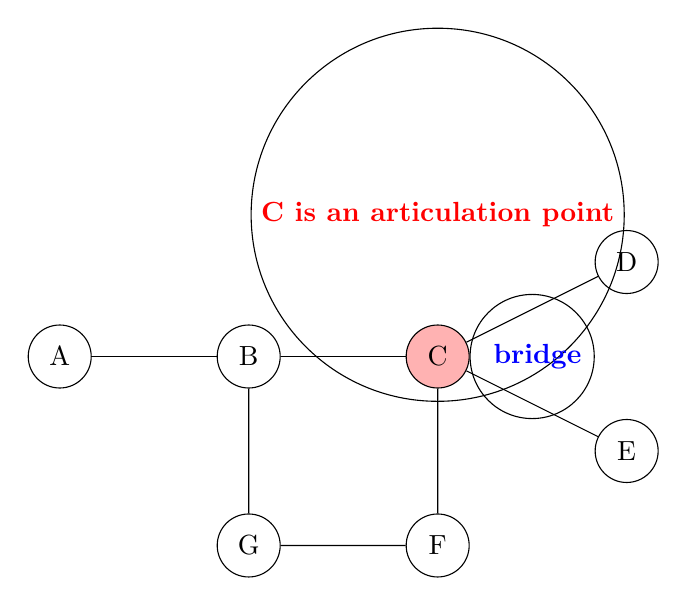
\begin{tikzpicture}[scale=1.2, every node/.style={circle, draw, minimum size=8mm}]
    % Nodes
    \node (A) at (0,0) {A};
    \node (B) at (2,0) {B};
    \node[fill=red!30] (C) at (4,0) {C}; % articulation point
    \node (D) at (6,1) {D};
    \node (E) at (6,-1) {E};
    \node (F) at (4,-2) {F};
    \node (G) at (2,-2) {G};

    % Edges
    \draw (A) -- (B);
    \draw (B) -- (C);
    \draw (C) -- (D);
    \draw (C) -- (E);
    \draw (C) -- (F);
    \draw (F) -- (G);
    \draw (G) -- (B);

    % Label
    \node at (4,1.5) {\textcolor{red}{\textbf{C is an articulation point}}};
    \node at (5,0) {\textcolor{blue}{\textbf{ bridge}}};
\end{tikzpicture}
\end{center}
\begin{minted}[
bgcolor=bgcolor1,
frame=lines,
framesep=5mm,
rulecolor=\color{black},
linenos,
numbersep=5pt,
fontsize=\normalsize
]{python}
from typing import List

def find_articulation_points(graph: dict, n: int) -> List[int]:
    """
    Finds articulation points in an undirected graph using DFS.
     Time Complexity: O(V+E)    Space Complexity: O(V)
    """
    
    ids = [-1] * n      # Discovery times of nodes
    low = [-1] * n      # Lowest ids reachable from a node
    visited = [False] * n
    is_articulation = [False] * n
    id_counter = 0      # Global id counter for assigning discovery times

    def dfs(node, parent, root):
        nonlocal id_counter
        visited[node] = True
        # Set the discovery time and low-link value
        ids[node] = low[node] = id_counter
        id_counter += 1
        children = 0  # Count of children in DFS tree

        for neighbor in graph.get(node, []):
            if neighbor == parent:
               continue   # Skip the edge back to the parent
            if not visited[neighbor]:
                children += 1
                dfs(neighbor, node, root)
                # Update low-link value based on child
                low[node] = min(low[node], low[neighbor])
                # If condition is met, node is an articulation point (not root)
                if ids[node] <= low[neighbor] and node != root:
                    is_articulation[node] = True

                # Special rule for root: it's an articulation point if it has >1 child
                if node == root and children > 1:
                    is_articulation[node] = True
            else:
                # Update low-link value due to back edge
                low[node] = min(low[node], ids[neighbor])

    for i in range(n):
        if not visited[i]:
            dfs(i, -1, i)
    return [i for i in range(n) if is_articulation[i]]
\end{minted} 

\noindent\textbf{Problem: Bridges in Graph (Tarjan's Algorithm)}
\begin{minted}[
bgcolor=bgcolor,
frame=lines,
framesep=5mm,
rulecolor=\color{black},
linenos,
numbersep=5pt,
fontsize=\normalsize
]{python}
def find_bridges(graph: dict, n: int) -> List[List[int]]:
    """
    Finds all bridges in undirected graph using DFS.
    Time Complexity: O(V+E)    Space Complexity: O(V)
    """
    ids = [-1] * n
    low = [-1] * n
    visited = [False] * n
    bridges = []
    id_counter = 0
    def dfs(node: int, parent: int):
        nonlocal id_counter
        visited[node] = True
        # Assign discovery time and low-link value
        ids[node] = low[node] = id_counter
        id_counter += 1

        # Explore neighbors
        for neighbor in graph.get(node, []):
            if neighbor == parent:
                # Don't revisit the edge we came from
                continue
            if not visited[neighbor]:
                # Recurse on unvisited neighbor
                dfs(neighbor, node)
                # Update low-link value
                low[node] = min(low[node], low[neighbor])

                # Bridge condition: no back-edge from neighbor or its subtree
                if ids[node] < low[neighbor]:
                    bridges.append([node, neighbor])
            else:
                # Update low-link value for back-edge
                low[node] = min(low[node], ids[neighbor])
    
    for i in range(n):
        if not visited[i]:
            dfs(i, -1)
    return bridges
\end{minted}

\noindent\textbf{Problem: Disjoint Set Union (DSU) with Path Compression}
\begin{minted}[
bgcolor=bgcolor10,
frame=lines,
framesep=5mm,
rulecolor=\color{black},
linenos,
numbersep=5pt,
fontsize=\normalsize
]{python}
class DSU:
    def __init__(self, n: int):
        self.parent = list(range(n))
        self.rank = [0] * n
        self.size = [1] * n  # Each node is its own set of size 1
    def find(self, x: int) -> int:
        """Finds root with path compression"""
        if self.parent[x] != x:
            self.parent[x] = self.find(self.parent[x])
        return self.parent[x]
    
    def union(self, x: int, y: int) -> bool:
        """Unions two sets, returns True if successful"""
        root_x = self.find(x)
        root_y = self.find(y)
        if root_x == root_y:
            return False  # Already connected
            
        # Union by rank
        if self.rank[root_x] < self.rank[root_y]:
            self.parent[root_x] = root_y
        elif self.rank[root_x] > self.rank[root_y]:
            self.parent[root_y] = root_x
        else:
            self.parent[root_y] = root_x
            self.rank[root_x] += 1
        return True
        
        def unionbysize(self, x, y):
        rootX = self.find(x)
        rootY = self.find(y)
        if rootX == rootY:
            return False  # Already in the same set
        # Union by size: attach smaller set under larger set
        if self.size[rootX] < self.size[rootY]:
            self.parent[rootX] = rootY
            self.size[rootY] += self.size[rootX]
        else:
            self.parent[rootY] = rootX
            self.size[rootX] += self.size[rootY]
        return True
\end{minted}

\noindent\textbf{Problem: Cycle Detection in Undirected Graph (DSU)}
\begin{minted}[
bgcolor=bgcolor5,
frame=lines,
framesep=5mm,
rulecolor=\color{black},
linenos,
numbersep=5pt,
fontsize=\normalsize
]{python}
def has_cycle_dsu(edges: List[tuple], n: int) -> bool:
    """
    Detects cycle in undirected graph using DSU.
    Time Complexity: O(E * Alpha(V)) Approx. O(E)    Space Complexity: O(V)
    """
    dsu = DSU(n)
    for u, v in edges:
        if not dsu.union(u, v):
            return True
    return False
\end{minted}

\noindent\textbf{Problem: Kruskal's MST Algorithm}
\begin{minted}[
bgcolor=bgcolor6,
frame=lines,
framesep=5mm,
rulecolor=\color{black},
linenos,
numbersep=5pt,
fontsize=\normalsize
]{python}
def kruskal_mst(edges: List[tuple], n: int) -> int:
    """
    Finds MST weight using Kruskal's algorithm with DSU.
    Time Complexity: O(E log E)    Space Complexity: O(V)
    """
    edges.sort(key=lambda x: x[2])  # Sort by weight
    dsu = DSU(n)
    mst_weight = 0
    
    for u, v, w in edges:
        if dsu.union(u, v):
            mst_weight += w
    return mst_weight
\end{minted}

\noindent\textbf{Problem: Word Ladder I (BFS)}
\begin{minted}[
bgcolor=bgcolor3,
frame=lines,
framesep=5mm,
rulecolor=\color{black},
linenos,
numbersep=5pt,
fontsize=\normalsize
]{python}
from collections import deque

def word_ladder(begin: str, end: str, word_list: List[str]) -> int:
    """
    Finds shortest transformation sequence length.
    Time Complexity: O(M^2 * N) where M=word length, N=word count
    Space Complexity: O(N)
    """
    word_set = set(word_list)
    if end not in word_set:
        return 0
        
    queue = deque([(begin, 1)])
    visited = set([begin])
    
    while queue:
        word, steps = queue.popleft()
        if word == end:
            return steps
            
        for i in range(len(word)):
            for c in 'abcdefghijklmnopqrstuvwxyz':
                next_word = word[:i] + c + word[i+1:]
                if next_word in word_set and next_word not in visited:
                    visited.add(next_word)
                    queue.append((next_word, steps + 1))
    return 0
\end{minted}

\noindent\textbf{Problem: 0/1 Matrix (Multi-source BFS)}
\begin{minted}[
bgcolor=bgcolor8,
frame=lines,
framesep=5mm,
rulecolor=\color{black},
linenos,
numbersep=5pt,
fontsize=\normalsize
]{python}
from collections import deque

def update_matrix(matrix: List[List[int]]) -> List[List[int]]:
    """
    Calculates distance to nearest 0 for each cell.
    Time Complexity: O(m*n)    Space Complexity: O(m*n)
    """
    m, n = len(matrix), len(matrix[0])
    dist = [[-1] * n for _ in range(m)]
    queue = deque()
    
    # Initialize queue with all 0s
    for i in range(m):
        for j in range(n):
            if matrix[i][j] == 0:
                dist[i][j] = 0
                queue.append((i, j))
    
    directions = [(1,0), (-1,0), (0,1), (0,-1)]
    while queue:
        x, y = queue.popleft()
        for dx, dy in directions:
            nx, ny = x + dx, y + dy
            if 0 <= nx < m and 0 <= ny < n and dist[nx][ny] == -1:
                dist[nx][ny] = dist[x][y] + 1
                queue.append((nx, ny))
    return dist
\end{minted}

\noindent\textbf{Problem: Surrounded Regions (DFS)}
\begin{minted}[
bgcolor=bgcolor5,
frame=lines,
framesep=5mm,
rulecolor=\color{black},
linenos,
numbersep=5pt,
fontsize=\normalsize
]{python}
def solve(board: List[List[str]]) -> None:
    """
    Flips surrounded 'O' to 'X' (in-place).
    Time Complexity: O(m*n)    Space Complexity: O(m*n)
    """
    if not board: return
    m, n = len(board), len(board[0])
    
    def dfs(i, j):
        if 0 <= i < m and 0 <= j < n and board[i][j] == 'O':
            board[i][j] = 'T'  # Temporary mark
            for dx, dy in [(1,0), (-1,0), (0,1), (0,-1)]:
                dfs(i+dx, j+dy)
    
    # Mark border-connected 'O's
    for i in range(m):
        dfs(i, 0)
        dfs(i, n-1)
    for j in range(n):
        dfs(0, j)
        dfs(m-1, j)
    
    # Flip inner 'O' to 'X' and restore border 'O's
    for i in range(m):
        for j in range(n):
            if board[i][j] == 'O':
                board[i][j] = 'X'
            elif board[i][j] == 'T':
                board[i][j] = 'O'
\end{minted}

\noindent\textbf{Problem: Is Graph Bipartite?}
\begin{minted}[
bgcolor=bgcolor2,
frame=lines,
framesep=5mm,
rulecolor=\color{black},
linenos,
numbersep=5pt,
fontsize=\normalsize
]{python}
def is_bipartite(graph: List[List[int]]) -> bool:
    """
    Checks if graph is bipartite using BFS coloring.
    Time Complexity: O(V+E)    Space Complexity: O(V)
    """
    n = len(graph)
    colors = [-1] * n  # -1: uncolored, 0/1: colors
    
    for i in range(n):
        if colors[i] == -1:
            queue = deque([i])
            colors[i] = 0
            while queue:
                node = queue.popleft()
                for neighbor in graph[node]:
                    if colors[neighbor] == -1:
                        colors[neighbor] = 1 - colors[node]
                        queue.append(neighbor)
                    elif colors[neighbor] == colors[node]:
                        return False
    return True
\end{minted}

\noindent\textbf{Problem: Find Eventual Safe States}
\begin{minted}[
bgcolor=bgcolor10,
frame=lines,
framesep=5mm,
rulecolor=\color{black},
linenos,
numbersep=5pt,
fontsize=\normalsize
]{python}
def eventual_safe_nodes(graph: List[List[int]]) -> List[int]:
    """
    Finds nodes that can reach terminal nodes (no cycles).
    Time Complexity: O(V+E)    Space Complexity: O(V)
    """
    n = len(graph)
    state = [0] * n  # 0: unvisited, 1: visiting, 2: safe
    
    def is_safe(node):
        if state[node] > 0:
            return state[node] == 2
        state[node] = 1  # mark as visiting
        for neighbor in graph[node]:
            if not is_safe(neighbor):  # if any neighbor leads to a cycle
                return False
        state[node] = 2  # mark as safe after exploring all neighbors
        return True
    return [i for i in range(n) if is_safe(i)]
    ###################################KAHN'S#########################################
def eventual_safe_nodes(graph: List[List[int]]) -> List[int]:
    """
    Finds eventual safe nodes using Kahn’s Algorithm (BFS + Topological Sort).
    Time Complexity: O(V + E)    Space Complexity: O(V + E)
    """
    n = len(graph)
    # Step 1: Reverse the graph
    reverse_graph = defaultdict(list)
    indegree = [0] * n
    for u in range(n):
        for v in graph[u]:
            reverse_graph[v].append(u)
            indegree[u] += 1  # original node u had an outgoing edge

    # Step 2: Start with terminal nodes (nodes with no outgoing edges originally)
    queue = deque([i for i in range(n) if indegree[i] == 0])
    safe = [False] * n  # Mark nodes proven to be safe
    while queue:
        node = queue.popleft()
        safe[node] = True
        for neighbor in reverse_graph[node]:  # Go in reversed direction
            indegree[neighbor] -= 1
            if indegree[neighbor] == 0:
                queue.append(neighbor)

    # Return sorted list of safe nodes
    return sorted([i for i, val in enumerate(safe) if val])

\end{minted}

\noindent\textbf{Problem: Alien Dictionary (Topo Sort)}
\begin{minted}[
bgcolor=bgcolor4,
frame=lines,
framesep=5mm,
rulecolor=\color{black},
linenos,
numbersep=5pt,
fontsize=\normalsize
]{python}
from collections import defaultdict, deque

def alien_order(words: List[str]) -> str:
    """
    Determines alien language order from sorted dictionary.
    Time Complexity: O(C) where C = total characters
    Space Complexity: O(1) fixed 26 letters
    """
    graph = defaultdict(set)
    indegree = defaultdict(int)
    all_chars = set(''.join(words))
    
    # Build graph and indegree
    for i in range(1, len(words)):
        a, b = words[i-1], words[i]
        min_len = min(len(a), len(b))
        for j in range(min_len):
            if a[j] != b[j]:
                if b[j] not in graph[a[j]]:
                    graph[a[j]].add(b[j])
                    indegree[b[j]] += 1
                break
        else:
            if len(a) > len(b):
                return ""  # Invalid
    
    # Kahn's algorithm
    queue = deque([c for c in all_chars if indegree.get(c, 0) == 0])
    order = []
    
    while queue:
        c = queue.popleft()
        order.append(c)
        for neighbor in graph[c]:
            indegree[neighbor] -= 1
            if indegree[neighbor] == 0:
                queue.append(neighbor)
    
    return ''.join(order) if len(order) == len(all_chars) else ""
\end{minted}

\noindent\textbf{Problem: Minimum Effort Path (BFS + Binary Search) And (Dijkstra)}
\begin{minted}[
bgcolor=bgcolor5,
frame=lines,
framesep=5mm,
rulecolor=\color{black},
linenos,
numbersep=5pt,
fontsize=\normalsize
]{python}
def minimum_effort_path(heights: List[List[int]]) -> int:
    """
    Finds min effort path (max abs diff) from top-left to bottom-right.
    Time Complexity: O(m*n*log(max_height))    Space Complexity: O(m*n)
    """
    m, n = len(heights), len(heights[0])
    low, high = 0, max(max(row) for row in heights)
    
    def can_reach(effort):
        visited = [[False] * n for _ in range(m)]
        queue = deque([(0,0)])
        visited[0][0] = True
        directions = [(1,0), (-1,0), (0,1), (0,-1)]
        
        while queue:
            x, y = queue.popleft()
            if x == m-1 and y == n-1:
                return True
            for dx, dy in directions:
                nx, ny = x+dx, y+dy
                if 0 <= nx < m and 0 <= ny < n and not visited[nx][ny]:
                    diff = abs(heights[x][y] - heights[nx][ny])
                    if diff <= effort:
                        visited[nx][ny] = True
                        queue.append((nx, ny))
        return False
    
    while low < high:
        mid = (low + high) // 2
        if can_reach(mid):
            high = mid
        else:
            low = mid + 1
    return low
                     #########################################

def minimum_effort_path(heights: List[List[int]]) -> int:
    """
    Dijkstra-based solution for minimum effort path.
    Each move has an 'effort' = abs height difference.
    We seek the path with minimum *maximum* effort along the path.
    """
    m, n = len(heights), len(heights[0])
    # Min-heap priority queue: (effort_so_far, x, y)
    heap = [(0, 0, 0)]    
    # Tracks minimum effort to reach each cell
    effort_to = [[float('inf')] * n for _ in range(m)]
    effort_to[0][0] = 0
    directions = [(-1, 0), (1, 0), (0, -1), (0, 1)]
    while heap:
        effort, x, y = heapq.heappop(heap)

        # If we reached bottom-right cell, return the effort
        if x == m - 1 and y == n - 1:
            return effort
        
        for dx, dy in directions:
            nx, ny = x + dx, y + dy
            if 0 <= nx < m and 0 <= ny < n:
                # Calculate effort to move to neighbor
                current_diff = abs(heights[nx][ny] - heights[x][y])
                max_effort = max(effort, current_diff)
                
                # If this path is better, update and add to heap
                if effort_to[nx][ny] > max_effort:
                    effort_to[nx][ny] = max_effort
                    heapq.heappush(heap, (max_effort, nx, ny))
    return -1  

\end{minted}

\noindent\textbf{Problem: Make a Large Island}
\begin{minted}[
bgcolor=bgcolor6,
frame=lines,
framesep=5mm,
rulecolor=\color{black},
linenos,
numbersep=5pt,
fontsize=\normalsize
]{python}
def largest_island(grid: List[List[int]]) -> int:
    """
    Finds largest island after changing at most one 0 to 1.
    Time Complexity: O(m*n)    Space Complexity: O(m*n)
    """
    m, n = len(grid), len(grid[0])
    island_id = 2  # Start from 2 (0/1 are used)
    area = defaultdict(int)
    directions = [(1,0), (-1,0), (0,1), (0,-1)]
    
    # DFS to mark islands and record areas
    def dfs(i, j, id):
        if 0 <= i < m and 0 <= j < n and grid[i][j] == 1:
            grid[i][j] = id
            count = 1
            for dx, dy in directions:
                count += dfs(i+dx, j+dy, id)
            return count
        return 0
    
    # Mark all islands and store their sizes
    for i in range(m):
        for j in range(n):
            if grid[i][j] == 1:
                area[island_id] = dfs(i, j, island_id)
                island_id += 1
    
    max_area = max(area.values()) if area else 0
    for i in range(m):
        for j in range(n):
            if grid[i][j] == 0:
                seen_ids = set()
                for dx, dy in directions:
                    ni, nj = i+dx, j+dy
                    if 0 <= ni < m and 0 <= nj < n and grid[ni][nj] > 1:
                        seen_ids.add(grid[ni][nj])
                total = 1 + sum(area[id] for id in seen_ids)
                max_area = max(max_area, total)
    return max_area
\end{minted}

\noindent\textbf{Problem: Cheapest Flights Within K Stops}
\begin{minted}[
bgcolor=bgcolor3,
frame=lines,
framesep=5mm,
rulecolor=\color{black},
linenos,
numbersep=5pt,
fontsize=\normalsize
]{python}
def find_cheapest_price(n: int, flights: List[List[int]], src: int, dst: int, k: int) -> int:
    """
    Finds cheapest flight with at most k stops using Bellman-Ford.
    Time Complexity: O(K * E)    Space Complexity: O(n)
    """
    prices = [float('inf')] * n
    prices[src] = 0
    
    # Relax edges k+1 times
    for _ in range(k+1):
        temp = prices[:]  # Copy current state
        for u, v, w in flights:
            if prices[u] != float('inf'):
                temp[v] = min(temp[v], prices[u] + w)
        prices = temp
    
    return prices[dst] if prices[dst] != float('inf') else -1
                     #########################################
def find_cheapest_price(n: int, flights: List[List[int]],src: int,dst: int,K: int) -> int:
    """
    Modified Dijkstra to find the cheapest flight with at most K stops.
    Uses (cost, node, stops) in the min-heap.
    """
    # Build adjacency list: u -> [(v, price)]
    graph = defaultdict(list)
    for u, v, price in flights:
        graph[u].append((v, price))
    
    # Min-heap: (total_cost, current_city, stops_so_far)
    heap = [(0, src, 0)]
    
    # Use a dict to track best cost at (city, stops)
    visited = dict()

    while heap:
        cost, city, stops = heapq.heappop(heap)
        # If destination reached within allowed stops, return the cost
        if city == dst:
            return cost
        # If already visited with fewer stops, skip (to avoid cycles and inefficiency)
        if (city, stops) in visited and visited[(city, stops)] <= cost:
            continue
        visited[(city, stops)] = cost

        # Only proceed if stops are within limit
        if stops <= K:
            for neighbor, price in graph[city]:
                new_cost = cost + price
                heapq.heappush(heap, (new_cost, neighbor, stops + 1))
    return -1
\end{minted}

\noindent\textbf{Problem: Number of Ways to Arrive at Destination}
\begin{minted}[
bgcolor=bgcolor,
frame=lines,
framesep=5mm,
rulecolor=\color{black},
linenos,
numbersep=5pt,
fontsize=\normalsize
]{python}
def count_paths(n: int, roads: List[List[int]]) -> int:
    """
    Counts number of shortest paths from 0 to n-1.
    Time Complexity: O(E log V)    Space Complexity: O(V)
    """
    MOD = 10**9 + 7
    graph = defaultdict(list)
    for u, v, time in roads:
        graph[u].append((v, time))
        graph[v].append((u, time))
    
    dist = [float('inf')] * n
    ways = [0] * n
    dist[0] = 0
    ways[0] = 1
    heap = [(0, 0)]
    
    while heap:
        d, node = heapq.heappop(heap)
        if d != dist[node]:
            continue
        for neighbor, time in graph[node]:
            new_dist = d + time
            if new_dist < dist[neighbor]:
                dist[neighbor] = new_dist
                ways[neighbor] = ways[node]
                heapq.heappush(heap, (new_dist, neighbor))
            elif new_dist == dist[neighbor]:
                ways[neighbor] = (ways[neighbor] + ways[node]) % MOD
    return ways[n-1] % MOD
\end{minted}
% \end{document}
